\subsection{Projection onto an arbitrary unit hypersphere}

\begin{figure}[ht]
    \centering
    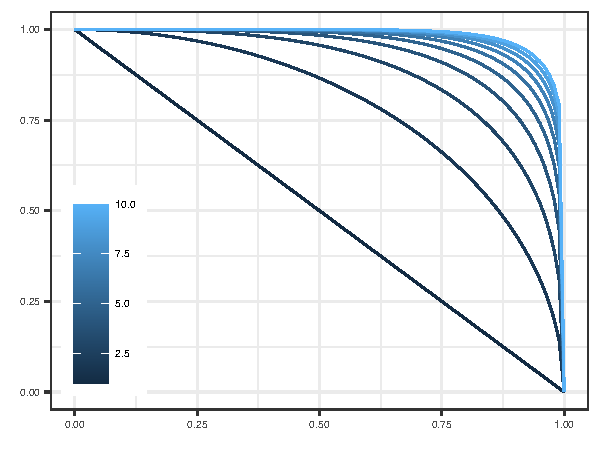
\includegraphics{images/p_sphere}
    \caption{Unit hyperspheres established on $\mathcal{L}_p$, for $p = 1,\ldots,10$, for two dimensions.\label{fig:psphere}}
\end{figure}

A hypersphere is a geometric object such that the distance from any point to the center takes a fixed,
  constant value.  The unit hypersphere is a hypersphere where that distance is 1. We can define the
  hypersphere under an arbitrary distance measurement, but for our purpose we will use the class of
  hyperspheres defined under the $\mathcal{L}_p$ norm. Let the $\mathcal{L}_p$-norm be defined as
  \begin{equation*}
    \lVert \bm{s} \rVert_p = \left({\textstyle\sum}_{l = 1}^d \lvert s_l\rvert^p\right)^{\frac{1}{p}}.
  \end{equation*}
  From this, we establish the $\mathcal{L}_1$ norm as $p = 1$, or the absolute sum; the
  $\mathcal{L}_2$ norm, as $p = 2$, the Euclidean distance.  From this we also establish the
  $\mathcal{L}_{\infty}$ norm, as
  \begin{equation*}
    \lVert \bm{s} \rVert_{\infty}
      = \lim\limits_{p\to\infty} \lVert \bm{s} \rVert_p
      = \max_{l\in\lbrace1,\ldots,d\rbrace}s_l.
  \end{equation*}
  We are interested in the direction, or angular component, of vectors described in the positive
  orthant, $\mathcal{R}_{+}^d$.  One means of describing the direction of a vector in $\mathcal{R}_+^d$
  is to project that vector onto $\mathcal{S}_{p}^{d-1}$, the positive orthant of the unit hypersphere
  defined on an $\mathcal{L}_p$-norm, denoted as $\mathcal{S}_{p}^{d-1}$.  That is,
  \begin{equation*}
    \mathcal{S}_{p}^{d-1} = \left\lbrace \bm{s} : \bm{s} \in \mathcal{R}_{+}^{d}, \lVert \bm{s}\rVert_{p} = 1\right\rbrace.
  \end{equation*}
  Figure~\ref{fig:psphere} shows $\mathcal{S}_{p}^{1}$ for $p$ at integers between 1 and 10.  At $p = 1$, we have the simplex.  As $p$ grows larger, the surface moves away from the origin and approaches closer to the unit hypercube--the limiting form of the surface. We project an observation onto $\mathcal{S}_p^{d-1}$ by dividing said observation by its $p$-norm--let  $\bm{x}\in \mathcal{R}_{+}^{d}$, then $\bm{y} = \bm{x} / \lVert \bm{x}\rVert_p \in \mathcal{S}_{p}^{d-1}$.
  We denote the $d-1$ to indicate the loss of one degree of freedom relative to the original vector.
  Observations on one hypersphere can be projected without loss of information onto another by
  dividing by the defining norm of the target hypersphere.
  
Assuming $\bm{y} \in \mathcal{S}_{p}^{d-1}$, then for finite $p$, $y_d$ can always be represented
  as a function of the other dimensions.  That is,
  \begin{equation*}
    y_d = \left(1 - {\textstyle\sum}_{l = 1}^{d-1}y_l^p\right)^{\frac{1}{p}}.
  \end{equation*}
  So the transformation
  \begin{equation}
    \label{eqn:pnormt}
    T(x_1,\ldots,x_d) = \left(\pnorm{\bm{x}}{p}, \frac{x_1}{\pnorm{\bm{x}}{p}},
                          \ldots , \frac{x_{d-1}}{\pnorm{\bm{x}}{p}}\right) = (r,y_1,\ldots,y_{d-1})
  \end{equation}
  does not lose any information.  The reverse of this transformation,
  \begin{equation}
    \label{eqn:pnormtinv}
    T^{-1}\left(r,y_1,\ldots,y_{d-1}\right) =
      \left(ry_1,\ldots,ry_{d-1}, r\left(1 - {\textstyle\sum}_{l = 1}^{d-1}y_l^p\right)^{\frac{1}{p}}\right)
  \end{equation}
  equivalently recovers the original data.  To recover the density of the transformed random variables,
  the original density is multiplied by the determinant of the Jacobian--the matrix of derivatives
  of the inverse transformation.  This takes the form:
  \begin{equation}
    \label{eqn:pnormjac}
    r^{d-1}\left[\left(1 - {\textstyle\sum}_{l = 1}^{d-1}y_l^p\right)^{\frac{1}{p}} +
        {\textstyle\sum}_{l = 1}^{d-1}y_l^p\left(1 - {\textstyle\sum}_{l=1}^{d-1} y_l^p\right)^{\frac{1}{p} - 1}\right].
  \end{equation}
  Notice a factor of $r^{d-1}$ independent of $p$. We refer to $\bm{y}$ and $r$ as, respectively,
  the angular and radial components of $\bm{x}$.  If we assume a distribution for $\bm{x}$, then
  by transforming to $r, \bm{y}$ and integrating out $r$, we are left with a distribution on solely
  $\bm{y}$, the projection of $\bm{x}$ onto $\mathcal{S}_{p}^{d-1}$.  If we take the projection to
  its limit as $p\to\infty$, we arrive at a projection onto $\mathcal{S}_{\infty}^{d-1}$.
  
We can observe a problem at this point in at least two ways.  First, on $\mathcal{S}_{\infty}^{d-1}$, the
  inverse transformation from $\mathcal{S}_{\infty}^{d-1}$ to $R_+^{d}$ in Equation~\ref{eqn:pnormtinv} 
  may not recover the original data--that formulation of the projection would only work when $Y_d = 1$.
  Alternatively, we may look at the formula for the determinant of the Jacobian in
  Equation~\ref{eqn:pnormjac}.  In that formula we observe the value 
  $(1 - \sum_{l = 1}^{d-1}y_l^p)^{\frac{1}{p} - 1}$.  As $p\to\infty$, 
  this quantity will go to $0^{-1}$ if $y_d \neq 1$.
  So, the mathematical basis of this transformation is thus dependent upon finite $p$.  However, we can
  project onto $\mathcal{S}_p^{d-1}$ for large $p$, and that projection will be similar to an idealized 
  distribution on $\mathcal{S}_{\infty}^{d-1}$.

% EOF
